\usetikzlibrary{calc,arrows.meta,patterns,angles,quotes}
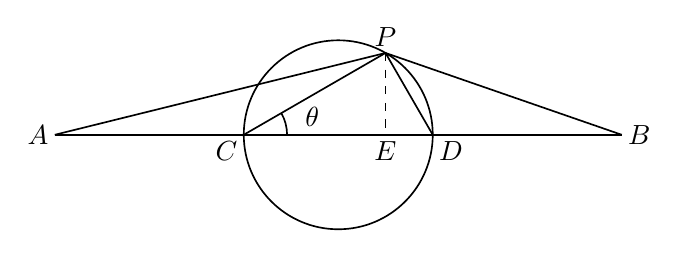
\begin{tikzpicture}[x=1cm,y=1cm,line width=.6pt,font=\normalsize,>=Stealth]
\coordinate (A) at (0.0000000000,0.0000000000);
\coordinate (C) at (2.4000000000,0.0000000000);
\coordinate (O) at (3.6000000000,0.0000000000);
\coordinate (D) at (4.8000000000,0.0000000000);
\coordinate (B) at (7.2000000000,0.0000000000);
\coordinate (P) at (4.2000000000,1.0392304845);
\coordinate (E) at (4.2000000000,0.0000000000);
\draw (O) circle[radius=1.2000000000cm];
\draw (A)--(B);
\draw (A)--(P);
\draw (B)--(P);
\draw (C)--(P);
\draw (D)--(P);
\draw[dashed] (P)--(E);
\draw (2.9500000000,0.0000000000) arc[start angle=0.0000000000,end angle=30.0000000000,radius=0.5500000000cm];
\node[left=2pt,inner sep=0pt] at (A) {$A$};
\node[right=2pt,inner sep=0pt] at (B) {$B$};
\node[below left=2pt,inner sep=0pt] at (C) {$C$};
\node[below right=2pt,inner sep=0pt] at (D) {$D$};
\node[below=2pt,inner sep=0pt] at (E) {$E$};
\node[above=2pt,inner sep=0pt] at (P) {$P$};
\node at (3.2693332437,0.2329371406) {$\theta$};
\end{tikzpicture}
